\documentclass[11pt]{article}

\usepackage{amsmath}
\usepackage{textcomp}
\usepackage[top=0.8in, bottom=0.8in, left=0.8in, right=0.8in]{geometry}
% Add other packages here %
\usepackage{color}
\usepackage{enumitem}
\usepackage{caption}
\usepackage{graphicx}
\usepackage{indentfirst}


\definecolor{pblue}{rgb}{0.13,0.13,1}
\definecolor{pgreen}{rgb}{0,0.5,0}
\definecolor{pred}{rgb}{0.9,0,0}
\definecolor{pgrey}{rgb}{0.46,0.45,0.48}

\usepackage{listings}
\lstset{language=Java,
  showspaces=false,
  showtabs=false,
  breaklines=true,
  showstringspaces=false,
  breakatwhitespace=true,
  commentstyle=\color{pgreen},
  keywordstyle=\color{pblue},
  stringstyle=\color{pred},
  basicstyle=\ttfamily,
  moredelim=[il][\textcolor{pgrey}]{$ $},
  moredelim=[is][\textcolor{pgrey}]{\%\%}{\%\%}
}

% Put your group number and names in the author field %
\title{\bf Excercise 1.\\ Implementing a first Application in RePast: A Rabbits Grass Simulation.}
\author{Group \textnumero 54: Oriol Barbany Mayor, Natalie Bolón Brun}

\begin{document}
\maketitle

\section{Implementation}

\subsection{Assumptions}
% Describe the assumptions of your world model and implementation (e.g. is the grass amount bounded in each cell) %
\subsubsection{Assumptions on the \textbf{agents}}

\textbf{Initial energy: }The initial energy of a rabbit, either when is born or when the simulation is initiated, is given by a random integer between 1 and the parameter of maximum initial energy named as \texttt{MaxEnergy}.
    
\textbf{Birth of a new rabbit: } Any rabbit whose energy reaches the \texttt{BirthThreshold} gives birth to a new rabbit. As a result, the parent's energy is reduced to one third of its current energy. We took this approach to avoid rabbits giving birth in two consecutive steps thus provoking an exponential growth in population.

\textbf{Position of rabbits: } A new rabbit can only be placed in a cell where there is currently no other rabbit. In the extreme case that the current space is completely full, the system does not allow the rabbits to move and/or reproduce anymore.
    
\textbf{Movement: } If a rabbit tries to move to a cell where there is currently another rabbit, the movement will be blocked and it will remain in its current place. 
    
\textbf{Energy: } For each time step, the energy of all rabbits is decreased by one unit regardless of their success in moving to a new cell. This way we avoid reaching a regime in which the map could be full of the same rabbits for infinitely many time. If the rabbit moves to a cell where there is grass, its energy will increase by the energetic value of the grass in that position. If the energy of an agent is 0 it will die, and therefore be removed from the system. Additionally, if its energy is equal or bigger that the birth threshold, it will give birth to a new rabbit as stated before.

\subsubsection{Assumptions on the \textbf{environment}}

\textbf{Initial grass energy: }The initial energy of each unit of new grass will be determined by a random integer between 1 and the parameter of maximum initial energy for grass named as \texttt{MaxGrassEnergy}.
    
\textbf{Position of grass: } Each new unit of grass is positioned in a random cell of the grid. If the cell already contains grass, their energetic values will be added and clipped to the maximum energy of the grass. Otherwise, the value of the cell will equal the energy of the grass.
    
\textbf{Grass spread: }The parameter \texttt{GrassGrowthRate} determines the number of cells which will be filled with grass at each step. Note that this is not necessarily equal to the number of new cells of grass for the above assumption.
    
\textbf{Torus space: }As stated in the problem description, the space is a torus. We will discuss its meaning in terms of implementation in section \ref{sec:imp-remarks}.



\subsection{Implementation Remarks}
% Provide important details about your implementation, such as handling of boundary conditions %

\subsubsection{Torus space}
\label{sec:imp-remarks}
At each step, we generate a proposal of a movement in NSEW randomly. We implement this by generating a random integer in $[1,4]$. On the one hand, when we have an ascending move in say axis $x$, we apply the modulus operator: \texttt{newX = (x + 1) \% grid.getSizeX();}. On the other hand, when the movement is descending we check if we reached a negative cell and if that's the case, we appear from the other side: \texttt{newX = ((x - 1) < 0) ? grid.getSizeX() - 1 : x - 1;}. Note that previous examples are respectively the same for the $y$ axis.

\subsubsection{Representations: grass' energy and rabbits}
In order to represent the level of energy that each unit of grass has, we create a bijection from an integer representing such energy to a green color with luminance proportional to it. Put differently, the brighter the green in a cell is, the more energy the grass has there. We thus have \texttt{MaxGrassEnergy} many green tonalities.

Rabbits are drawn using the library \texttt{uchicago.src.sim.gui.SimGraphics}, and specifically with the function \texttt{drawHollowFastOval} in white color. We chose this as it only draws a white ring and the transparent background allows to see whether the rabbit is stepping on grass or not.

\section{Results}
% In this section, you study and describe how different variables (e.g. birth threshold, grass growth rate etc.) or combinations of variables influence the results. Different experiments with diffrent settings are described below with your observations and analysis

\subsection{Experiment 1}
\subsubsection{Setting}

Default parameters are shown in Table \ref{tab:exp1}.

\subsubsection{Observations}

\begin{minipage}[]{\textwidth}

\begin{minipage}[]{0.2\textwidth}
\resizebox{\textwidth}{!}{%
\begin{tabular}{|l|l|}
\hline
\textbf{Parameter} & \textbf{Value} \\ \hline
\textbf{Birth Threshold} & 15 \\ \hline
\textbf{Grass Growth Rate} & 10 \\ \hline
\textbf{Grid Size} & 20 \\ \hline
\textbf{Max Energy} & 20 \\ \hline
\textbf{Max Grass Energy} & 5 \\ \hline
\textbf{Num Init Rabbits} & 10 \\ \hline
\textbf{Num Init Grass} & 10 \\ \hline
\end{tabular}%
}
\captionof{table}{Default parameters.}
\label{tab:exp1}
\end{minipage}{}
\hfill
\begin{minipage}[]{0.75\textwidth}
Given the previous parameters, we see that the population of rabbits increases from the initial value until reaching a value around which it oscillates. The grass quantity evolves similarly, increasing its energetic content until a point around which it oscillates. Both variables behave symmetrically interchanging energy while maintaining the energy of the system constant.   
\end{minipage}{}

\end{minipage}{}

\subsection{Experiment 2}
\subsubsection{Setting}
Influence of \texttt{BirthThreshold} and \texttt{GridSize}. Remaining parameters keep their default values. Both parameters are modified independently and result in the same behaviour.

\subsubsection{Observations}
We can distinguish 3 cases: for $\texttt{BirthThreshold} \leq 5$, the population of rabbits explodes and may reach the maximum capacity of the system. Most of the rabbits have low energetic content while a few ones accumulate a great amount of energy. For $5 < \texttt{BirthThreshold} \leq 35$, the population of rabbits increases but the energetic content of the system remains mostly concentrated on the grass. Energy along rabbits is distributed following a normal distribution with mean lower than the birth threshold. Finally, for $35 < \texttt{BirthThreshold}$, the population stabilizes around a value and its energetic content is greater than the grass system. The population of rabbits is constituted of individuals with very high energetic content. Cases 2 and 3 are shown in Figure \ref{fig:exp1}.

\begin{minipage}[]{\textwidth}

\begin{minipage}[]{0.5\textwidth}
\begin{minipage}[]{\textwidth}
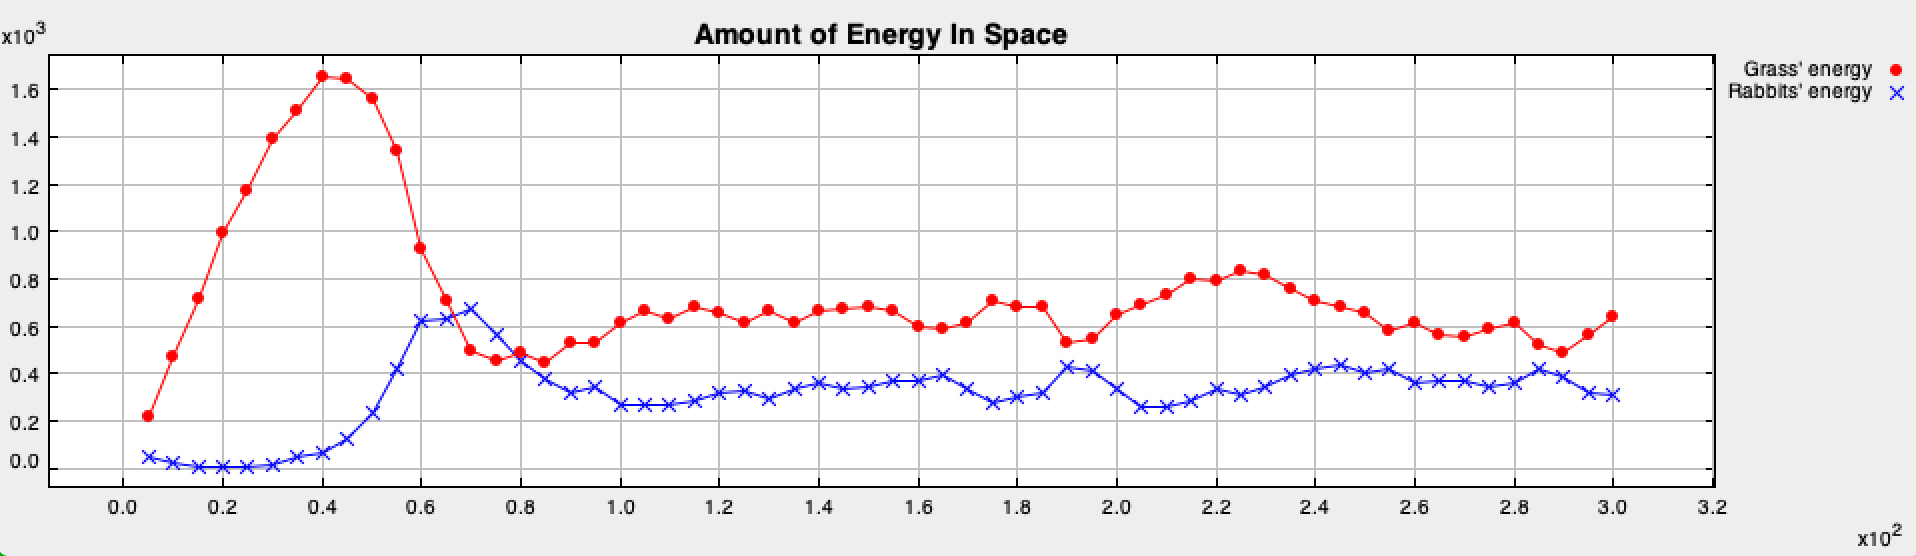
\includegraphics[width=\textwidth]{1-rabbits/Images-report/evolution-20.png}
\end{minipage}
\hfill
\begin{minipage}[]{\textwidth}
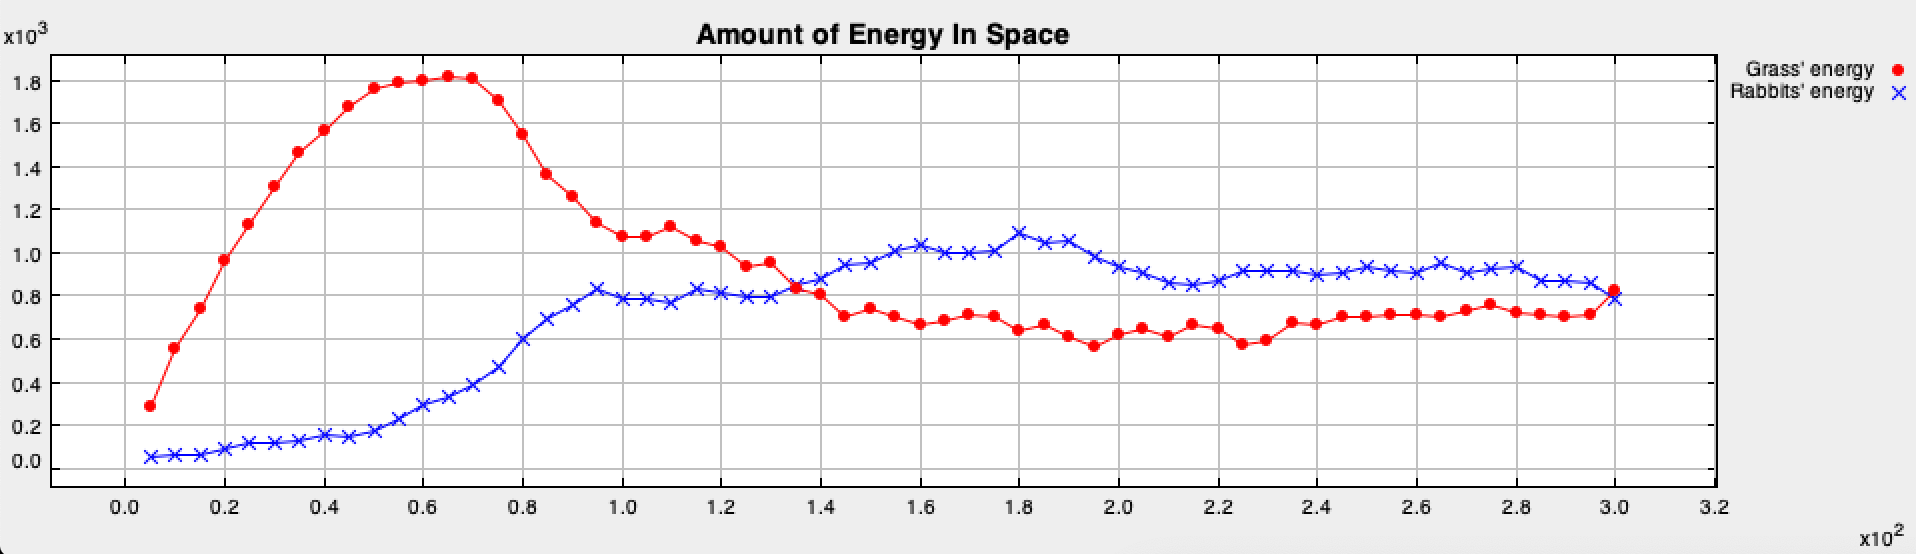
\includegraphics[width=\textwidth]{1-rabbits/Images-report/evolution-50.png}
\captionof{figure}{From top to bottom: \texttt{BirthThreshold}= 20 and 50}
\label{fig:exp1}
\end{minipage}{}

\end{minipage}{}
\hfill
\begin{minipage}[]{0.35\textwidth}
 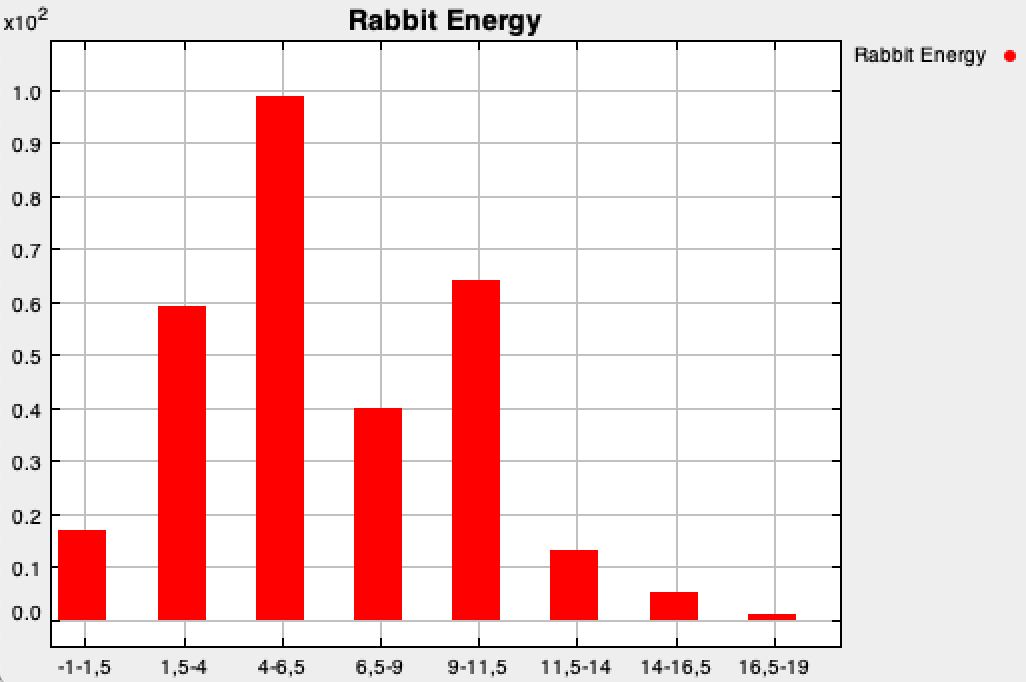
\includegraphics[width=\textwidth]{1-rabbits/Images-report/rabbit-energy-150.png}
\captionof{figure}{\texttt{GrassGrowthRate}=60. Step = 150. Alive rabbits = 298}
\label{fig:exp2}
\end{minipage}{}

\end{minipage}{}

\subsection{Experiment 3}
\subsubsection{Setting}

Influence of \texttt{MaxGrassEnergy}, \texttt{MaxEnergy} and \texttt{GrassGrowthRate}. Remaining parameters keep their default values. All parameters are modified independently. 

\subsubsection{Observations}

For $\texttt{MaxGrassEnergy} \leq 3$ the population of rabbits extinguishes at an early stage of the simulation since the available grass is not energetic enough to allow the continuation of the species. Grass continues growing until reaching its maximum energetic level in around 250 steps. For $\texttt{MaxGrassEnergy} > 3$ the population survives. Once reached this state, the energy is distributed among grass and rabbits forcing a symmetric behaviour of these two values around the equilibrium.

Initially, the energetic content of the grass is higher than the one of the rabbits. As we increase the studied parameter, this gap becomes smaller until the point when \texttt{MaxGrassEnergy} equals \texttt{MaxEnergy} when both groups stabilize around a point with similar energetic content.

Modifying \texttt{MaxEnergy} has the same effect as \texttt{MaxGrassEnergy} but in this case, if the parameter keeps increasing, the energetic gap grows and the rabbits become the group holding the greatest amount of energy in the system. 

Modifying \texttt{GrassGrowthRate} effects in the same way. As we increase the parameter the gap of energetic content between grass and rabbits' populations increases. The population of rabbits increases but the energy of each individual remains low (under 10u) as seen in Figure \ref{fig:exp2}.

\subsection{Experiment 4} 
\subsubsection{Setting}
Influence of \texttt{NumInitGrass} and \texttt{NumInitRabbits}. Remaining parameters keep their default values. Each parameter is modified independently. 
\subsubsection{Observations}
We have found no influence on the system for \texttt{NumInitGrass} while \texttt{NumInitRabbits} produces the same behaviour as when varying \texttt{GrassGrowthRate}. 


\end{document}